\section{Kodo-python}

\subsection{Exercise 0:}
It took about 20 minutes to get the product installing once the license was granted. The process to acquire the license could have been easier than signing up for a license using a google docs template. Even though Steinwurf quickly responded with permission we did not get a Github Notification as we assumed we would. Then a couple days later when we wanted to install the library we couldn't figure out how to get access. After a while we found a mail that granted me access. This was the part that took the most time. We guess if the process of granting permissions to the repositories had been smoother, the experience would have been better.

The installation process was fairly simple for people accustomed to computer terminals. On a mac it was go to the cloned repository in the terminal and execute to command and that almost it. To use and thus verify the installation the guide suggests two ways of doing so. Either copy the kodo.so file to the folder or add it to Python Path. We ended up copying the file, even though we found the other solution the most elegant one, however we couldn't get it to work.

\begin{figure}[H]
    \centering
    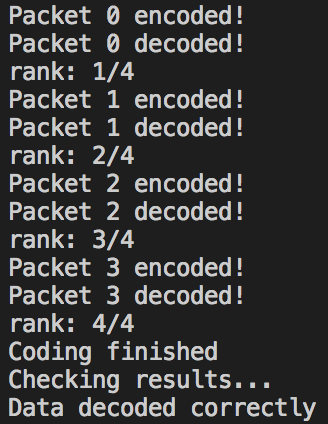
\includegraphics[width=0.2\textwidth]{figures/KodoPython/encode_decode.png}
    \caption{Encode and Decode}
    \label{fig:encode_decode}
\end{figure}

\subsection{Exercise 1:}
\begin{figure}[H]
    \centering
    \begin{subfigure}{.49\textwidth}
        \centering
        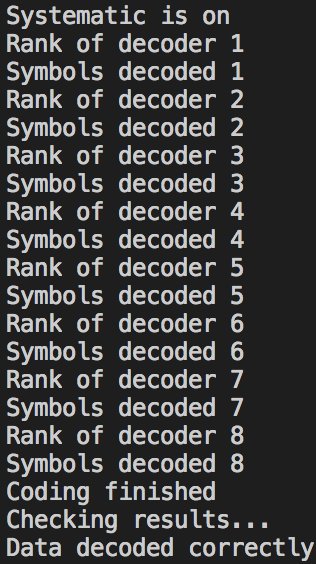
\includegraphics[width=0.4\textwidth]{figures/KodoPython/systematic_on.png}
        \caption{Systematic On}
        \label{fig:systematic_on}
    \end{subfigure}
    \begin{subfigure}{.5\textwidth}
        \centering
        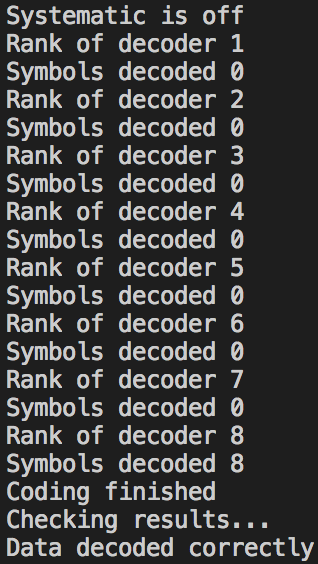
\includegraphics[width=0.4\textwidth]{figures/KodoPython/systematic_off.png}
        \caption{Systematic Off}
        \label{fig:systematic_off}
    \end{subfigure}
    \caption{Systematic On/Off}
    \label{fig:systematic_on_off}
\end{figure}
\textbf{Questions}
\begin{enumerate}
    \item \textit{Identify how many packets the encoder must generate, for the decoder to decode the data, with systematic mode ON and OFF.}\\ 
    Systematic mode on requires only 1 package to decode. The encoder sends the uncoded symbols, when getting a previously uncoded symbol\\
    Systematic mode off requires all packages to decode. The decoder must figure out how to decode the symbols itself.\\
    \textit{ - Do you need to increase the amount of coded packages generate to decode the data with systematic mode OFF?}\\
    YES! See above
    \item \textit{Identify if changes in g and k affect the number of packages generated. Note down your configurations for g and k.}\\
    The number of packages equals g.
    \item \textit{Based, on your knowledge of RLNC, Storage Systems, and Systematic Mode, is systematic mode a beneficial thing or not? In either case argue why.}\\
    It depends on the requirements for the system. It's a trade-off between network traffic and computation time.
\end{enumerate}

\subsection{Exercise 2:}
We have altered the setup a bit, for every value of g, we have tested with k=8...131072.

\begin{figure}[H]
    \centering
    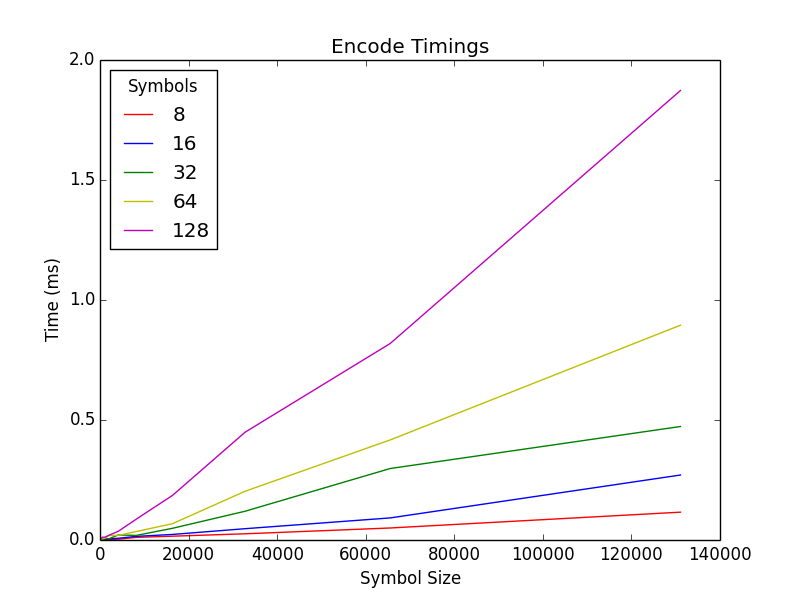
\includegraphics[width=0.7\textwidth]{figures/KodoPython/encode_timings.png}
    \caption{Encode Timings}
    \label{fig:encode_timings}
\end{figure}
\begin{figure}[H]
    \centering
    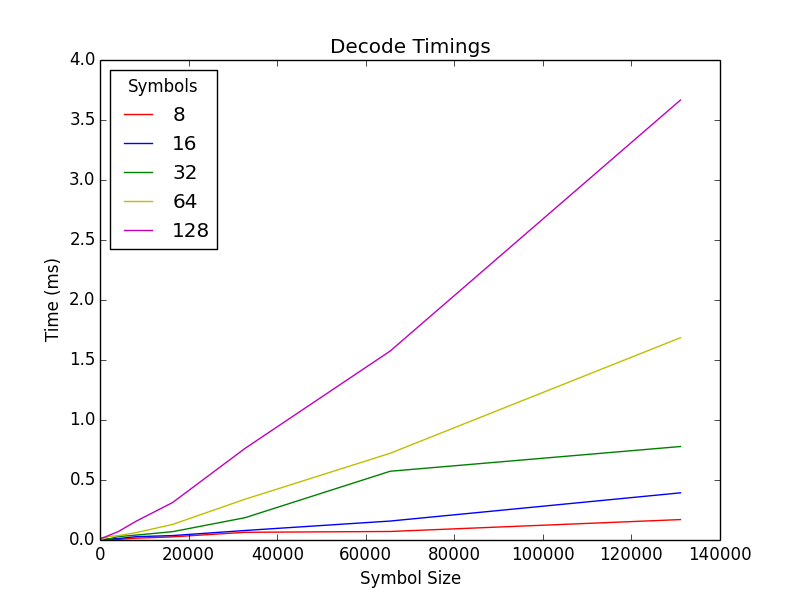
\includegraphics[width=0.7\textwidth]{figures/KodoPython/decode_timings.png}
    \caption{Encode Timings}
    \label{fig:decode_timings}
\end{figure}

The test shows that when g increase with a factor of 2 so does the time of computation.
For higher values of g the bigger impact k has on the computation time, for both encoding and decoding. 

\subsection{Exercise 3:}
Using the supplied Python and image, we have answered the following quiestions:
\begin{enumerate}
    \item \textit{How many clouds can you take down before it becomes impossible to decode the image.}\\
    Our setup: g=128, k=1024, 5 redundancy and 20 clouds.
    We vary the loss percentage of clouds crashes in increments of 10\%. We are not able to recreate the file from 60\% cloud crashes and upwards.
    \item \textit{Does the configuration for g and k effect the above. Choose your own g and k.}\\
    We altered the storage\_simulation.py to return true/false by comparing the initial image with the restored one.
    We've chosen to simulate with 50\% and 60\% cloud losses as this is the area where the recreation gets problematic.
    We setup main.py to run simulations with varying g and k, the results are given in table \cref{tab:Exercise3}.
    The results show that for small g and k the clouds are not able to recreate the file.
    \begin{table}[H]
        \begin{tabularx}{\textwidth}{|Y|Y|Y|Y|}
            \hline
            \cellcolor{gray}g & \cellcolor{gray}k & \cellcolor{gray}50\% Loss & \cellcolor{gray}60\% Loss \\\hline
            \cellcolor{lightgray}64 & \cellcolor{lightgray}1024 & \textcolor{red}{False}& \textcolor{red}{False}\\\hline
            \cellcolor{lightgray}64 & \cellcolor{lightgray}2048 & \textcolor{green}{True} & \textcolor{red}{False}\\\hline
            \cellcolor{lightgray}64 & \cellcolor{lightgray}4096 & \textcolor{green}{True} & \textcolor{green}{True}\\\hline
            \cellcolor{lightgray}64 & \cellcolor{lightgray}8192 & \textcolor{green}{True} & \textcolor{green}{True}\\\hline
            \cellcolor{lightgray}64 & \cellcolor{lightgray}16384 & \textcolor{green}{True} & \textcolor{green}{True}\\\hline
            \cellcolor{lightgray}128 & \cellcolor{lightgray}1024 & \textcolor{green}{True} & \textcolor{red}{False}\\\hline
            \cellcolor{lightgray}128 & \cellcolor{lightgray}2048 & \textcolor{green}{True} & \textcolor{green}{True}\\\hline
            \cellcolor{lightgray}128 & \cellcolor{lightgray}2096 & \textcolor{green}{True} & \textcolor{green}{True}\\\hline
            \cellcolor{lightgray}128 & \cellcolor{lightgray}8192 & \textcolor{green}{True} & \textcolor{green}{True}\\\hline
            \cellcolor{lightgray}128 & \cellcolor{lightgray}16384 & \textcolor{green}{True} & \textcolor{green}{True}\\\hline
        \end{tabularx}
        \caption{Picture recreation success}
        \label{tab:Exercise3}
    \end{table}

    \item \textit{Reflect on what you observe}\\
    Increaing g and k adds further redundancy to the storage system by trading-off the file sizes and thus the storage capacity.  
    
\end{enumerate}

\subsection{Exercise 4:}
\underline{\textit{Why RLNC should/shouldn't be used in distributed storage, and if you see an alternative:}}\\
First and foremost RLNC can be used to provide reliability in cloud setups. Our setup showed the critical point for
fault tolerance is above 50\%, which is descent enough. 
However, we have only tested when it's critical   

\subsection{Reflection}
The library was easy enough to use for this exercise. However, to do it from scratch probably would have been more troublesome due to lack of API description.
We encountered a problem running the storage simulator for g < 64 and k < 1024. The problem did not occur at all with g and k above the mentioned.

\pagebreak